\documentclass[10pt,a4paper]{article}
\usepackage[margin=1.6cm]{geometry}
\usepackage{graphicx}
\usepackage{booktabs}
\usepackage{microtype}
\usepackage{hyperref}
\usepackage{amsmath}
\usepackage{xcolor}
\usepackage{float}
\setlength{\parskip}{2pt}
\setlength{\parindent}{0pt}

\title{\vspace{-2em}Feature Tracking and Dynamic Object Detection}
\author{Mahdi Gheysari, Filippo Businaro, Riccardo Pesce}
\date{\vspace{-1em}April 2026}

\begin{document}
\maketitle
\vspace{-2em}

\section{The problem}

We have five short video sequences. In each one, a single object
moves: a bird, a car, a frog, a sheep, a squirrel. We have to
look at the first frame and draw a box around the moving object.
We cannot use deep learning, only classical computer vision. The
output is a text file with the box (\texttt{xmin ymin xmax ymax})
and an image with the box drawn on it.

We watched the videos first. In four sequences the camera does
not move, in the car sequence it pans a little to the right.

\section{Our method}

The idea is simple. If we put points on the first frame and
follow them, the points on the background do not move much (or
all move with the camera) and the points on the object move
differently. We just have to find the points that move
differently and put a box around them. Everything is done with
\textbf{OpenCV~4}.

\textbf{Step 1 -- CLAHE.} Some videos are dark, like the frog.
We apply local histogram equalisation to every frame so the next
step can find points on dim or smooth surfaces. We use a small
clip limit of $0.5$ on $8\times8$ tiles, which is gentle enough
not to add noise on already-bright scenes.
OpenCV: \texttt{cv::createCLAHE}, \texttt{clahe->apply}.

\textbf{Step 2 -- Find good corners.} A good point is a corner:
a place where the image changes a lot in two directions. We ask
for up to $1500$ corners on the equalised first frame.
OpenCV: \texttt{cv::goodFeaturesToTrack(gray, p0, 1500, 0.005, 5)}.
The quality $0.005$ is small enough to keep corners on the
squirrel fur, big enough so the grass does not flood the result.

\textbf{Step 3 -- Follow the corners with optical flow.} For each
later frame we ask: where did each point go? We use pyramidal
Lucas--Kanade. It looks at a small window around each point and
matches it in the next frame; the pyramid means it works even
when the point moves a lot. We also do a forward--backward check:
flow from $t$ to $t{+}1$, then from $t{+}1$ back to $t$. If the
point does not return close to where it started, we throw it
away.
OpenCV: \texttt{cv::calcOpticalFlowPyrLK} (window $21\times21$, $3$
pyramid levels), called twice for the two directions.

\textbf{Step 4 -- Remove the camera.} For each frame we take the
median of the surviving points' movements. The median is the
camera. We subtract it. Background points now have almost zero
movement, object points still move. The median is robust: even
if half the points are on the object, the other half is on the
background and the median picks the background.

\textbf{Step 5 -- Pick the moving points.} For each track we
compute the average leftover motion across all frames. We sort
and keep the top $15\%$, but only if their motion is bigger than
$\max(8\,\text{px}, 4\times\text{median})$. The floor throws
away small fake motions like leaves in the wind, distant
walkers, or animals that almost do not move.

\textbf{Step 6 -- Draw the box.} We have the moving points. We
group them by distance (a simple DBSCAN-style rule), take the
biggest group, throw away outliers with median absolute deviation,
and take the bounding rectangle with a small padding ($1/6$ of the
box size on each side, because corners sit inside the object not on
the silhouette). A small extra step uses pixel differences to
shrink the box if it is clearly too big: we shift each later frame
back to frame~0 with \texttt{cv::phaseCorrelate} and
\texttt{cv::warpAffine}, take \texttt{cv::absdiff} with frame~0,
threshold with Otsu (\texttt{cv::threshold} +
\texttt{THRESH\_OTSU}), clean it with \texttt{cv::morphologyEx}, and
take the largest blob with
\texttt{cv::connectedComponentsWithStats}. We only accept this
shrink when the new box is much smaller than the old one.

\textbf{What we tried first.} Our first version used \textbf{SIFT}
features matched between frame 0 and every later frame with
Lowe's ratio test. It worked for the car and the sheep but failed
on the squirrel: it is small (about $1\%$ of the image) and its
fur does not have stable SIFT points, so we got IoU $0.31$, below
the $0.5$ threshold. We changed to optical flow because it does
not need a perfect SIFT keypoint, only a corner the tracker can
follow.

\section{Results}

\begin{table}[H]
\centering\small
\begin{tabular}{lcccc}
\toprule
category & GT (w$\times$h) & ours & IoU & TP@0.5 \\
\midrule
bird     & $283\times255$ & $249\times241$ & 0.578 & yes \\
car      & $68\times42$   & $75\times 48$  & 0.773 & yes \\
frog     & $133\times 98$ & $98\times 83$  & 0.532 & yes \\
sheep    & $321\times179$ & $333\times195$ & 0.796 & yes \\
squirrel & $23\times31$   & $28\times 37$  & 0.616 & yes \\
\midrule
\multicolumn{3}{r}{\textbf{mIoU}}         & \textbf{0.659} & \\
\multicolumn{3}{r}{\textbf{accuracy@0.5}} & \textbf{1.00} & (5/5) \\
\bottomrule
\end{tabular}
\end{table}

\textbf{Bird, car, sheep} are the easy cases: many strong corners
on each object, Lucas--Kanade follows them, the moving ones are
clear and the box covers most of the object.

\textbf{Squirrel} is the smallest object. With SIFT we failed (IoU
$0.31$). With Shi--Tomasi corners we find only $5$ moving points
but they all sit on the squirrel, so the box is correct
(IoU $0.62$).

\textbf{Frog} is where CLAHE helps a lot. Without CLAHE the body
is too smooth and dark, the corner detector finds points only on
the legs and the branch (IoU $0.28$). After CLAHE the body gets
contrast, more corners land on the back and sides, the box covers
the body and IoU goes up to $0.53$.

\begin{figure}[H]
\centering
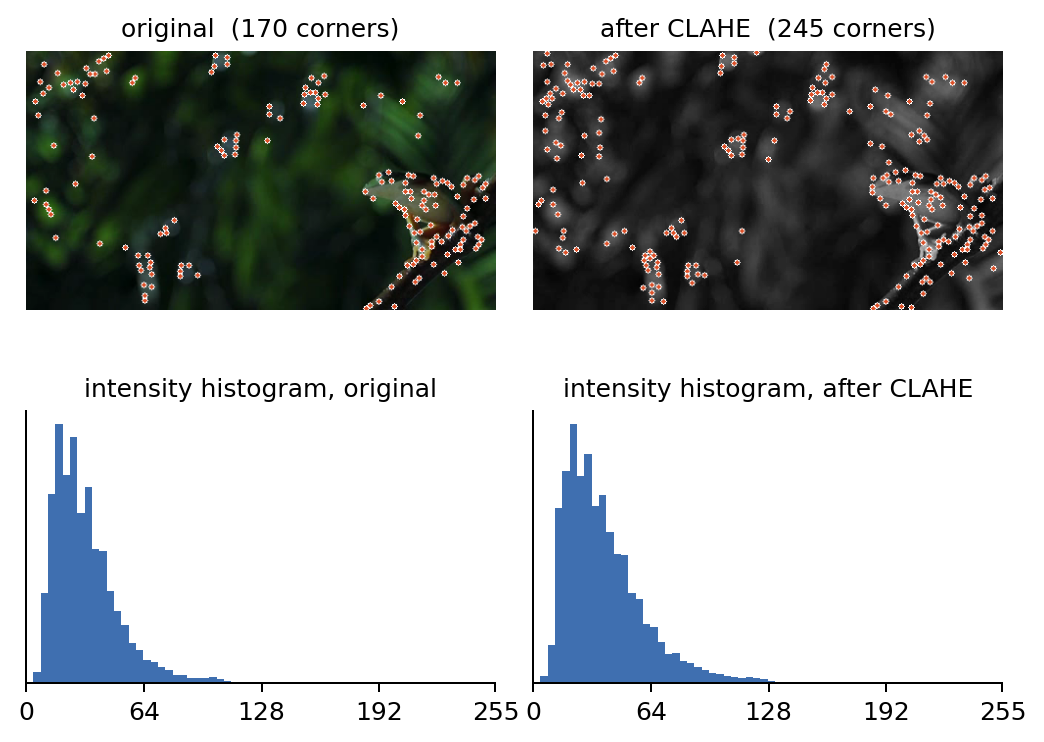
\includegraphics[width=0.78\linewidth]{figures/frog_clahe.png}
\caption{Frog frame 0 before and after CLAHE. Original: $170$
corners, equalised: $245$. The new corners are on the body. The
histograms show CLAHE spreading the dark pixels into a wider
range.}
\end{figure}

\begin{figure}[H]
\centering
\setlength{\tabcolsep}{3pt}
\begin{tabular}{ccc}
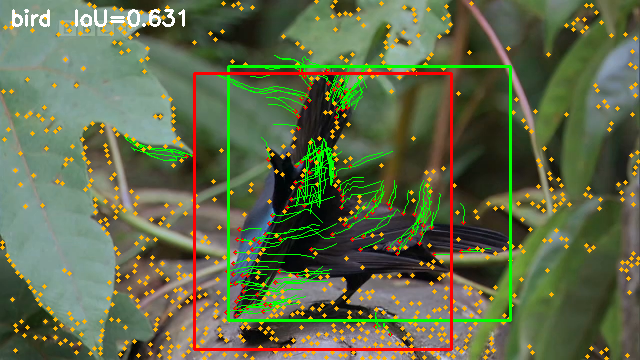
\includegraphics[width=0.31\linewidth]{figures/bird_overlay.png} &
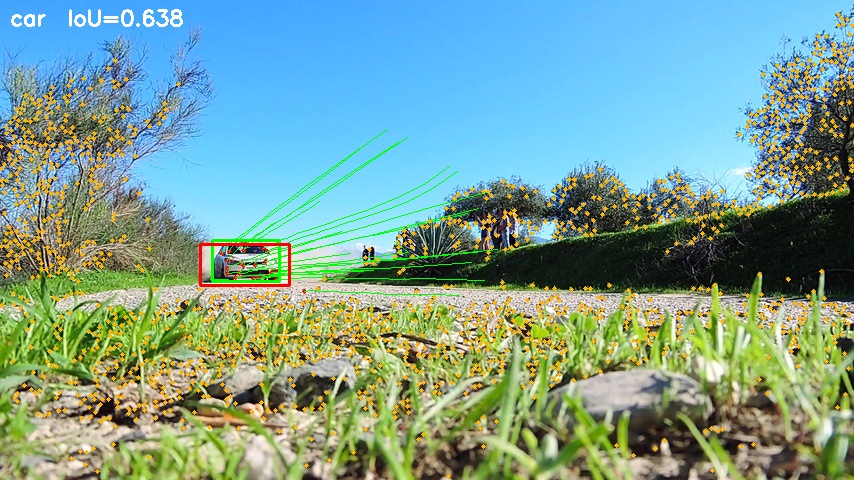
\includegraphics[width=0.31\linewidth]{figures/car_overlay.png} &
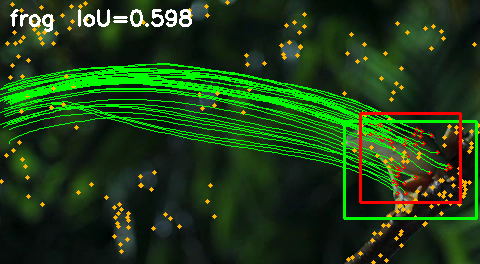
\includegraphics[width=0.31\linewidth]{figures/frog_overlay.png} \\
{\footnotesize bird} & {\footnotesize car} & {\footnotesize frog} \\[4pt]
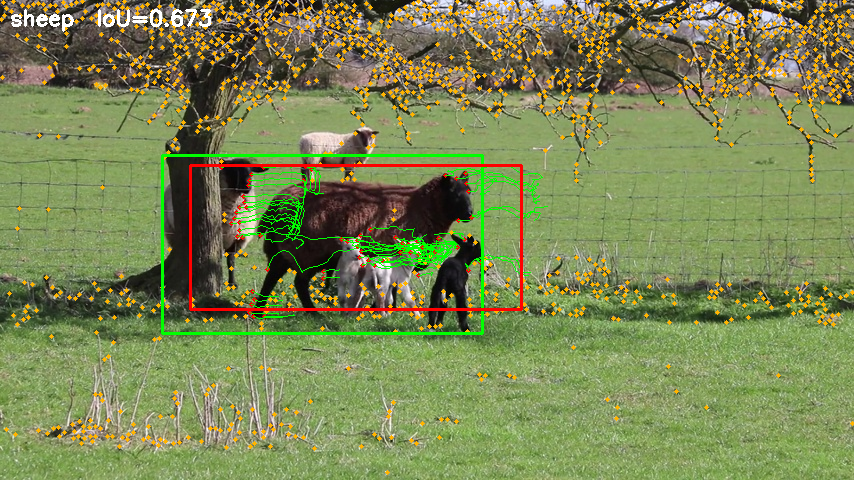
\includegraphics[width=0.31\linewidth]{figures/sheep_overlay.png} &
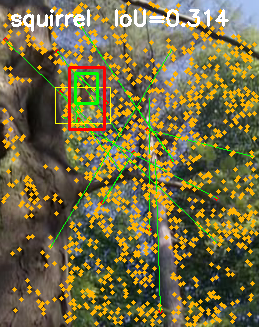
\includegraphics[width=0.31\linewidth]{figures/squirrel_overlay.png} & \\
{\footnotesize sheep} & {\footnotesize squirrel} & \\
\end{tabular}
\caption{First frame of each video. Green: ground truth. Red:
our prediction. Orange dots: detected corners on frame 0. Green
lines: trajectories of corners classified as moving.}
\end{figure}

\section{Code and people}

\textbf{Layout.} \texttt{src/feature\_tracker.cpp} (CLAHE +
corners + Lucas--Kanade + median camera removal),
\texttt{motion\_segmenter.cpp} (which points are moving),
\texttt{bbox\_estimator.cpp} (group + box),
\texttt{silhouette\_refiner.cpp} (optional shrink),
\texttt{evaluator.cpp} (IoU), \texttt{main.cpp} (driver),
\texttt{include/dod.hpp}, \texttt{CMakeLists.txt}. Build:
\texttt{cmake -S . -B build \&\& cmake --build build}. Run:
\texttt{./build/detect dataset output}. Only OpenCV~4.

\textbf{Who did what.} Mahdi Gheysari --
\texttt{feature\_tracker.cpp}, \texttt{main.cpp}.
Filippo Businaro -- \texttt{motion\_segmenter.cpp},
\texttt{silhouette\_refiner.cpp}, \texttt{evaluator.cpp}.
Riccardo Pesce -- \texttt{bbox\_estimator.cpp},
\texttt{include/dod.hpp}. Design choices, parameter tuning and
the report were shared. Total time around $32$ hours.

\end{document}
